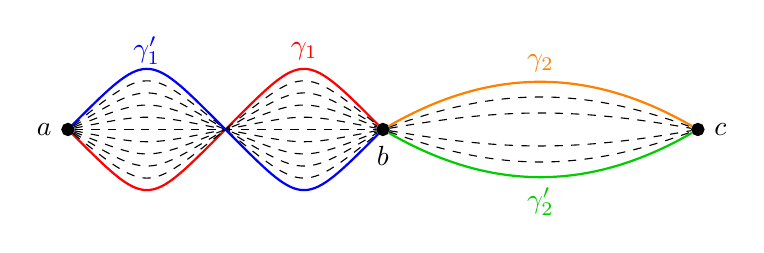
\begin{tikzpicture}
    \tikzstyle{point}=[circle,thick,draw=black,fill=black,inner sep=0pt,minimum width=4pt,minimum height=4pt]
    \node at (3,1) [red] {$\gamma_1$};
    \node at (1,1) [blue] {$\gamma_1'$};
    \node (a)[point,label=180:$a$] at (0,0) {};
    \node (b)[point,label=-90:$b$]   at (4, 0) {};
    \node (c)[point,label=0:$c$]   at (8, 0) {};
    \draw [rounded corners, thick, red] (a) .. controls (1,-1) .. (2,0)  .. controls (3,1) .. (b);
    \draw [rounded corners, dashed] (a) .. controls (1,-0.8) .. (2,0) .. controls (3,0.8) .. (b);
    \draw [rounded corners, dashed] (a) .. controls (1,-0.6) .. (2,0) .. controls (3,0.6) .. (b);
    \draw [rounded corners, dashed] (a) .. controls (1,-0.4) .. (2,0) .. controls (3,0.4) .. (b);
    \draw [rounded corners, dashed] (a) .. controls (1,-0.2) .. (2,0) .. controls (3,0.2) .. (b);
    \draw [rounded corners, dashed] (a) .. controls (1,   0) .. (2,0) .. controls (3,0.0) .. (b);
    \draw [rounded corners, dashed] (a) .. controls (1, 0.2) .. (2,0) .. controls (3,-0.2) .. (b);
    \draw [rounded corners, dashed] (a) .. controls (1, 0.4) .. (2,0) .. controls (3,-0.4) .. (b);
    \draw [rounded corners, dashed] (a) .. controls (1, 0.6) .. (2,0) .. controls (3,-0.6) .. (b);
    \draw [rounded corners, dashed] (a) .. controls (1, 0.8) .. (2,0) .. controls (3,-0.8) .. (b);
    \draw [rounded corners, dashed] (a) .. controls (1, 1.0) .. (2,0) .. controls (3,-1.0) .. (b);
    \draw [rounded corners, thick, blue] (a) .. controls (1,1) .. (2,0) .. controls (3,-1) .. (b);
    \draw [rounded corners, thick, green!80!black] (b) edge[bend right] node[below] {$\gamma_2'$} (c);
    \draw [rounded corners, dashed] (b) edge[bend right=20] (c);
    \draw [rounded corners, dashed] (b) edge[bend right=-20] (c);
    \draw [rounded corners, dashed] (b) edge[bend right=10] (c);
    \draw [rounded corners, dashed] (b) edge[bend right=-10] (c);
    \draw [rounded corners, thick, orange] (b) edge[bend left] node[above] {$\gamma_2$} (c);
\end{tikzpicture}
